\documentclass{acmsiggraph}               % final
%\documentclass[review]{acmsiggraph}      % review
%\documentclass[widereview]{acmsiggraph}  % wide-spaced review
%\documentclass[preprint]{acmsiggraph}    % preprint

%% Uncomment one of the four lines above depending on where your paper is
%% in the conference process. ``review'' and ``widereview'' are for review
%% submission, ``preprint'' is for pre-publication, and ``final'' is for
%% the version to be printed.

%% These two line bring in essential packages: ``mathptmx'' for Type 1 
%% typefaces, and ``graphicx'' for inclusion of EPS figures.

\usepackage{mathptmx}
\usepackage{graphicx}

%% use this for zero \parindent and non-zero \parskip, intelligently.

\usepackage{parskip}

%% If you are submitting a paper to the annual conference, please replace 
%% the value ``0'' below with your OnlineID. If you are not submitting this
%% paper to the annual conference, you may safely leave it at ``0'' -- it 
%% will not be included in the output.

\onlineid{0}

%% need to document this!

\acmformat{print}

%% Paper title.

\title{Segmentation for Fun and Profit}

%% Author and Affiliation (single author).

\author{Devin Smith\thanks{e-mail: dsmith@hmc.edu}\\Harvey Mudd College}


%% Keywords that describe your work.

\keywords{clustering, segmentation, sketch}

%%%%%% START OF THE PAPER %%%%%%

\begin{document}

\teaser{
  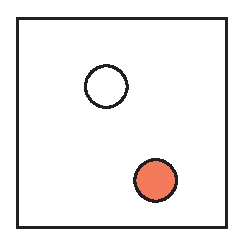
\includegraphics[width=1.5in]{sample.eps}
  \caption{Lookit! Lookit!}
}

%% The ``\maketitle'' command must be the first command after the
%% ``\begin{document}'' command. It prepares and prints the title block.

\maketitle

\section{Problem Statement}

%% The ``\copyrightspace'' command must be the first command after the 
%% start of the first section of the body of your paper. It ensures the
%% copyright space is left at the bottom of the first column on the first
%% page of your paper.

\copyrightspace

\section{Related Work}

\begin{figure}[h]
\centering
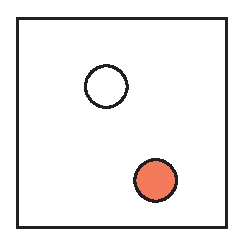
\includegraphics[width=1.5in]{sample.eps}
\caption{Sample illustration.}
\end

\section{Approach}

\section{Results and Discussion}


\section{Future Work}


\section{Conclusion}


\bibliographystyle{acmsiggraph}
\nocite{*}
\bibliography{template}
\end{document}
